%% 
%% Copyright 2019-2020 Elsevier Ltd
%% 
%% This file is part of the 'CAS Bundle'.
%% --------------------------------------
%% 
%% It may be distributed under the conditions of the LaTeX Project Public
%% License, either version 1.2 of this license or (at your option) any
%% later version.  The latest version of this license is in
%%    http://www.latex-project.org/lppl.txt
%% and version 1.2 or later is part of all distributions of LaTeX
%% version 1999/12/01 or later.
%% 
%% The list of all files belonging to the 'CAS Bundle' is
%% given in the file `manifest.txt'.
%% 
%% Template article for cas-dc documentclass for 
%% double column output.

%\documentclass[a4paper,fleqn,longmktitle]{cas-dc}
\documentclass[a4paper,fleqn]{cas-sc}

%\usepackage[numbers]{natbib}
%\usepackage[authoryear]{natbib}
\usepackage[authoryear,longnamesfirst]{natbib}
\usepackage{graphicx}
\usepackage{caption}
\usepackage{subcaption}

%%%Author definitions
\def\tsc#1{\csdef{#1}{\textsc{\lowercase{#1}}\xspace}}
\tsc{WGM}
\tsc{QE}
\tsc{EP}
\tsc{PMS}
\tsc{BEC}
\tsc{DE}
%%%

% Uncomment and use as if needed
%\newtheorem{theorem}{Theorem}
%\newtheorem{lemma}[theorem]{Lemma}
%\newdefinition{rmk}{Remark}
%\newproof{pf}{Proof}
%\newproof{pot}{Proof of Theorem \ref{thm}}

\begin{document}
\let\WriteBookmarks\relax
\def\floatpagepagefraction{1}
\def\textpagefraction{.001}

% Short title
\shorttitle{Two-Mode Relational Similarities}

% Short author
%\shortauthors{O. Lizardo}

% Main title of the paper
\title [mode = title]{Two-Mode Relational Similarities}                      
% Title footnote mark
% eg: \tnotemark[1]
%\tnotemark[1,2]

% Title footnote 1.
% eg: \tnotetext[1]{Title footnote text}
% \tnotetext[<tnote number>]{<tnote text>} 
%\tnotetext[1]{}

%\tnotetext[2]{.}


% First author
%
% Options: Use if required
% eg: \author[1,3]{Author Name}[type=editor,
%       style=chinese,
%       auid=000,
%       bioid=1,
%       prefix=Sir,
%       orcid=0000-0000-0000-0000,
%       facebook=<facebook id>,
%       twitter=<twitter id>,
%       linkedin=<linkedin id>,
%       gplus=<gplus id>]
\author[1]{Omar Lizardo}[orcid=0000-0001-7511-2910]

% Corresponding author indication
\cormark[1]

% Footnote of the first author
\fnmark[1]

% Email id of the first author
\ead{olizardo@soc.ucla.edu}

% URL of the first author
\ead[url]{http://olizardo.bol.ucla.edu/}

%  Credit authorship
\credit{Conceptualization of this study, Methodology, Software}

% Address/affiliation
\affiliation[1]{organization={University of California, Los Angeles},
    addressline={264 Haines Hall}, 
    city={Los Angeles},
    %citysep={}, % Uncomment if no comma needed between city and postcode
     postcode={90095}, 
     state={CA},
     country={USA}}

% Corresponding author text
\cortext[cor1]{Corresponding author}
%\cortext[cor2]{Principal corresponding author}

% Footnote text
\fntext[fn1]{This paper was written while the author was partially supported by National Science Foundation grant HNDS-R \#2214215.}
 % author as well.}
%\fntext[fn2]{Another author footnote, this is a very long footnote and
 % it should be a really long footnote. But this footnote is not yet
 % sufficiently long enough to make two lines of footnote text.}

% For a title note without a number/mark
%\nonumnote{This note has no numbers. In this work we demonstrate $a_b$
%  the formation Y\_1 of a new type of polariton on the interface
 % between a cuprous oxide slab and a polystyrene micro-sphere placed
 % on the slab.
 % }
% Here goes the abstract
\begin{abstract}
In a previous paper, Kovacs \citeyearpar{kovacs2010} proposed a generalized relational similarity measure based on iterated correlations of entities in a network calibrated by their relational similarity to other entities. Here I show that, in the case of two-mode network data, Kovacs's approach can be simplified and generalized similarities calculated non-iteratively. The basic idea is to rely on initial similarities calculated from transforming the two-mode data into one-mode projections using the familiar duality approach due to Breiger \citeyearpar{breiger1974}. I refer to this as two-mode relational similarities and show, using the Southern Women data, that it yields results substantively indistinguishable from Kovacs's, and, in some ways, more interpretable. 
\end{abstract}

% Use if graphical abstract is present
% \begin{graphicalabstract}
% 
\includegraphics{figs/grabs.pdf}
% \end{graphicalabstract}

 Research highlights
\begin{highlights}
    \item Previous work has developed measures of generalized similarity based on iterated correlations for two-mode data.
    \item This paper proposes a non-iterative measure of generalized similarity for two-mode data based on the projection approach.
    \item The paper shows that the two-mode relational similarity performs as well as the iterative correlations approach. 
\end{highlights}

% Keywords
% Each keyword is separated by \sep
\begin{keywords}
Generalized similarity \sep Duality \sep Two-mode networks \sep Correlation distance \sep Projection
\end{keywords}


\maketitle
\newpage

\section{Introduction}
In a previous paper, Kovacs \citeyearpar{kovacs2010} introduced a generalized relational similarity measure based on iterated correlations applicable to two-mode and one-mode network data. According to Kovacs, a desirable generalized similarity measure must have two desirable properties. First, (1) it should respect the \textit{principle of equivalence}, such that it classifies actors as similar if they have similar relations to other objects who are themselves similar Second, (2) the similarity measure should respect the \textit{principle of duality} \citep{breiger1974}, such that it classifies actors as similar if they have similar relations to similar objects, and objects as similar if they have similar relations to similar actors within the same system. 

Kovacs's key observation is that such a generalized relational similarity measure could be obtained by transforming the usual correlation distance measure. Particularly, Kovacs begins by noting that in the two-mode case, the correlation distance between any pair of actors $D(A)^{cor}_{i,j}$ be expressed as a function of their row profiles in actors $\times$ objects affiliation matrix $\mathbf{M}$ as follows:

\begin{equation}
    D(A)^{cor}_{i,j} = 
    \frac{
    (M_{i\bullet} - \bar{M_{i\bullet}})
    (M_{j\bullet} - \bar{M_{j\bullet}})^T
    }
    {
    \sqrt{
    (M_{i\bullet} - \bar{M_{i\bullet}})
    (M_{i\bullet} - \bar{M_{i\bullet}})^T
    (M_{j\bullet} - \bar{M_{j\bullet}})
    (M_{j\bullet} - \bar{M_{j\bullet}})^T
        }
    }
    \label{eq:1}
\end{equation}

Where $M_{i\bullet}$ is the row profile corresponding to actor $i$, $M_{j\bullet}$ is the row profile corresponding to actor $j$, $\bar{M_{i\bullet}}$ is the row mean for actor $i$, and $\bar{M_{j\bullet}}$ is the row mean for actor $j$ in the affiliation matrix. The same approach can be used to find the correlation distance between any two column objects $D(O)^{cor}_{i, j}$, by substituting their column profiles $(M_{\bullet i}, M_{\bullet j})$ and column means $(\bar{M_{\bullet i}}, \bar{M_{\bullet j})}$ into equation \ref{eq:1}. Overall, increasingly positive values of the correlation distance indicate actor similarity, while negative values  indicate actor dissimilarity, with values bounded in the $(-1, 1)$ interval.

Kovacs noted that the correlation distance classifies actors as similar if they have similar relations to other objects, but fails to incorporate the inter-object similarities. That is, actors should receive more similarity ``points'' if they connect to objects that are themselves similar. To this end, consider a matrix $\mathbf{S(O)}$ with cell entries $s(o)_{ij}$ capturing pairwise similarities between the objects in the two-mode network. In this case, a generalized relational similarity (GRS) measure for actors based on the correlation distance can be expressed as:

\begin{equation}
    D(A)^{grs}_{i,j} = 
    \frac{
    (M_{i\bullet} - \bar{M_{i\bullet}})
    \mathbf{S(O)}
    (M_{j\bullet} - \bar{M_{j\bullet}})^T
    }
    {
    \sqrt{
    (M_{i\bullet} - \bar{M_{i\bullet}})
    \mathbf{S(O)}
    (M_{i\bullet} - \bar{M_{i\bullet}})^T
    }
    \sqrt{
    (M_{j\bullet} - \bar{M_{j\bullet}})
    \mathbf{S(O)}
    (M_{j\bullet} - \bar{M_{j\bullet}})^T
        }
    }
    \label{eq:2}
\end{equation}

Kovacs notes that if we have access to an analogous matrix of similarities between actors $\mathbf{S(A)}$ in the network, then we would be able to also calculate a generalized relational similarity score for objects $D(O)_{grs}$ by plugging in that matrix and the column profiles and means into equation \ref{eq:2}, yielding:

\begin{equation}
    D(O)^{grs}_{i,j} = 
    \frac{
    (M_{\bullet i} - \bar{M_{\bullet i}})
    \mathbf{S(A)}
    (M_{\bullet i} - \bar{M_{\bullet i}})^T
    }
    {
    \sqrt{
    (M_{\bullet i} - \bar{M_{\bullet i}})
    \mathbf{S(A)}
    (M_{\bullet i} - \bar{M_{\bullet i}})^T
    }
    \sqrt{
    (M_{\bullet j} - \bar{M_{\bullet j}})
    \mathbf{S(A)}
    (M_{\bullet j} - \bar{M_{\bullet j}})^T
        }
    }
    \label{eq:3}
\end{equation}

Typically, people only have access to the network information and not exogenous indication of pre-existing similarities between actors or objects, required to compute \ref{eq:2}, and \ref{eq:3}. Kovacs's (ingenious) solution is to use the duality property and compute ``reflective similarities'' by first computing initial object similarities by plugging $D(A)_{cor}$ into \ref{eq:3} (equivalent to substituting the identity matrix, of dimensions $O \times O$, into the slot occupied by $\mathbf{S(O)}$ in \ref{eq:2}). Then using the resulting actor similarities to compute generalized object similarities. This is done by substituting a $A \times A$ matrix of $D(A)_{grs}$ values obtained in the first step into the slot occupied by $\mathbf{S(A)}$ in \ref{eq:3}. The iterations continue until both $D(A)_{grs}$ and $D(A)_{grs}$ ``freeze'' according to some stopping criterion ($\epsilon$). 

\section{Two-Mode Relational Similarities}
The basic purpose of this comment is to show that there is a simpler alternative to the iteration approach to computing generalized relational similarities in two-mode data. This alternative respects the basic spirit of Kovacs's proposal, namely, the principles of equivalence and duality, while exploiting the duality of actors and objects in two-mode networks more directly.

The basic idea is that similarity matrices that can play the role of $\mathbf{S(A)}$ and $\mathbf{S(O)}$ can be obtained from any two-mode network without iteration. Instead, they can be computed via Breiger's \citeyearpar{breiger1974} well-known dual projection approach (see also \citep{everett2013}). 

This procedure has two major steps. First, we obtain actor co-membership ($\mathbf{AA}$) and object overlap matrices ($\mathbf{OO}$) from the affiliation matrix ($\mathbf{M}$) following the well-known formulas:

\begin{equation}
    \mathbf{AA} = \mathbf{MM^T}
    \label{eq:4}
\end{equation}


\begin{equation}
    \mathbf{OO} = \mathbf{M^TM}
    \label{eq:5}
\end{equation}

For both $\mathbf{AA}$ and $\mathbf{OO}$, the $ij^{th}$ entry is the number of objects shared by actors $i$ and $j$ and the number of actors who choose both objects $i$ and $j$ respectively. The diagonal entries in $AA_{ij}$ record the number of objects each actor chooses, and the diagonal entries in $OO_{ij}$ record the number of actors choosing each object. 

Once we have these one-mode projections, it is straightforward to compute similarity measures across actors based on their co-memberships and across objects in terms of the actors they share. The basic idea is that the similarity between actors increases as the number of common objects chosen increases, and the similarity between objects increases as the number of actors who choose both objects, suitably weighted by both actors ``expansiveness" and object ``popularity" (the diagonal entries of $\mathbf{AA}$ and $\mathbf{OO}$, respectively). 

Many options are available here (and the results are invariant to this choice), but the cosine similarity is a straightforward candidate \citep{goodman1996single} For actors, this is given by:

\begin{equation}
    S(A)^{cos}_{ij} = \frac{AA_{ij}}{\sqrt{AA_{ii}AA_{jj}}}
    \label{eq:6}
\end{equation}

And for objects:

\begin{equation}
    S(O)^{cos}_{ij} = \frac{OO_{ij}}{\sqrt{OO_{ii}OO_{jj}}}
    \label{eq:7}
\end{equation}

We can then compute a distance matrix containing relational similarities between actors and objects directly without iteration, which I refer to as \textit{two-mode relationality similarity}. 

For actors, this is:

\begin{equation}
    D(A)^{tmrs}_{i,j} = 
    \frac{
    (M_{i\bullet} - \bar{M_{i\bullet}})
    \mathbf{S(O)^{cos}}
    (M_{j\bullet} - \bar{M_{j\bullet}})^T
    }
    {
    \sqrt{
    (M_{i\bullet} - \bar{M_{i\bullet}})
    \mathbf{S(O)^{cos}}
    (M_{i\bullet} - \bar{M_{i\bullet}})^T
    }
    \sqrt{
    (M_{j\bullet} - \bar{M_{j\bullet}})
    \mathbf{S(O)^{cos}}
    (M_{j\bullet} - \bar{M_{j\bullet}})^T
        }
    }
    \label{eq:8}
\end{equation}

And correspondingly, for objects, this is given by:

\begin{equation}
    D(O)^{tmrs}_{i,j} = 
    \frac{
    (M_{\bullet i} - \bar{M_{\bullet i}})
    \mathbf{S(A)^{cos}}
    (M_{\bullet i} - \bar{M_{\bullet i}})^T
    }
    {
    \sqrt{
    (M_{\bullet i} - \bar{M_{\bullet i}})
    \mathbf{S(A)^{cos}}
    (M_{\bullet i} - \bar{M_{\bullet i}})^T
    }
    \sqrt{
    (M_{\bullet j} - \bar{M_{\bullet j}})
    \mathbf{S(A)^{cos}}
    (M_{\bullet j} - \bar{M_{\bullet j}})^T
        }
    }
    \label{eq:9}
\end{equation}

Where everything is as before. It is easy to see that equations \ref{eq:8} and \ref{eq:9} respect the principle of equivalence. Actors count as similar to the extent they connect to similar objects ($\mathbf{S(O)^{cos}}$). Conversely, objects count as similar to the extent they are chosen by similar actors ($ \mathbf{S(A)^{cos}}$). Because the similarities are defined according to the dual projection method, in which the similarity of actors is based on the objects they choose, and the similarity of objects is based on the actors who choose them, the measure also respects the principle of duality.

\begin{figure}[ht!]
     \begin{subfigure}[b]{1.0\textwidth}
        \centering
        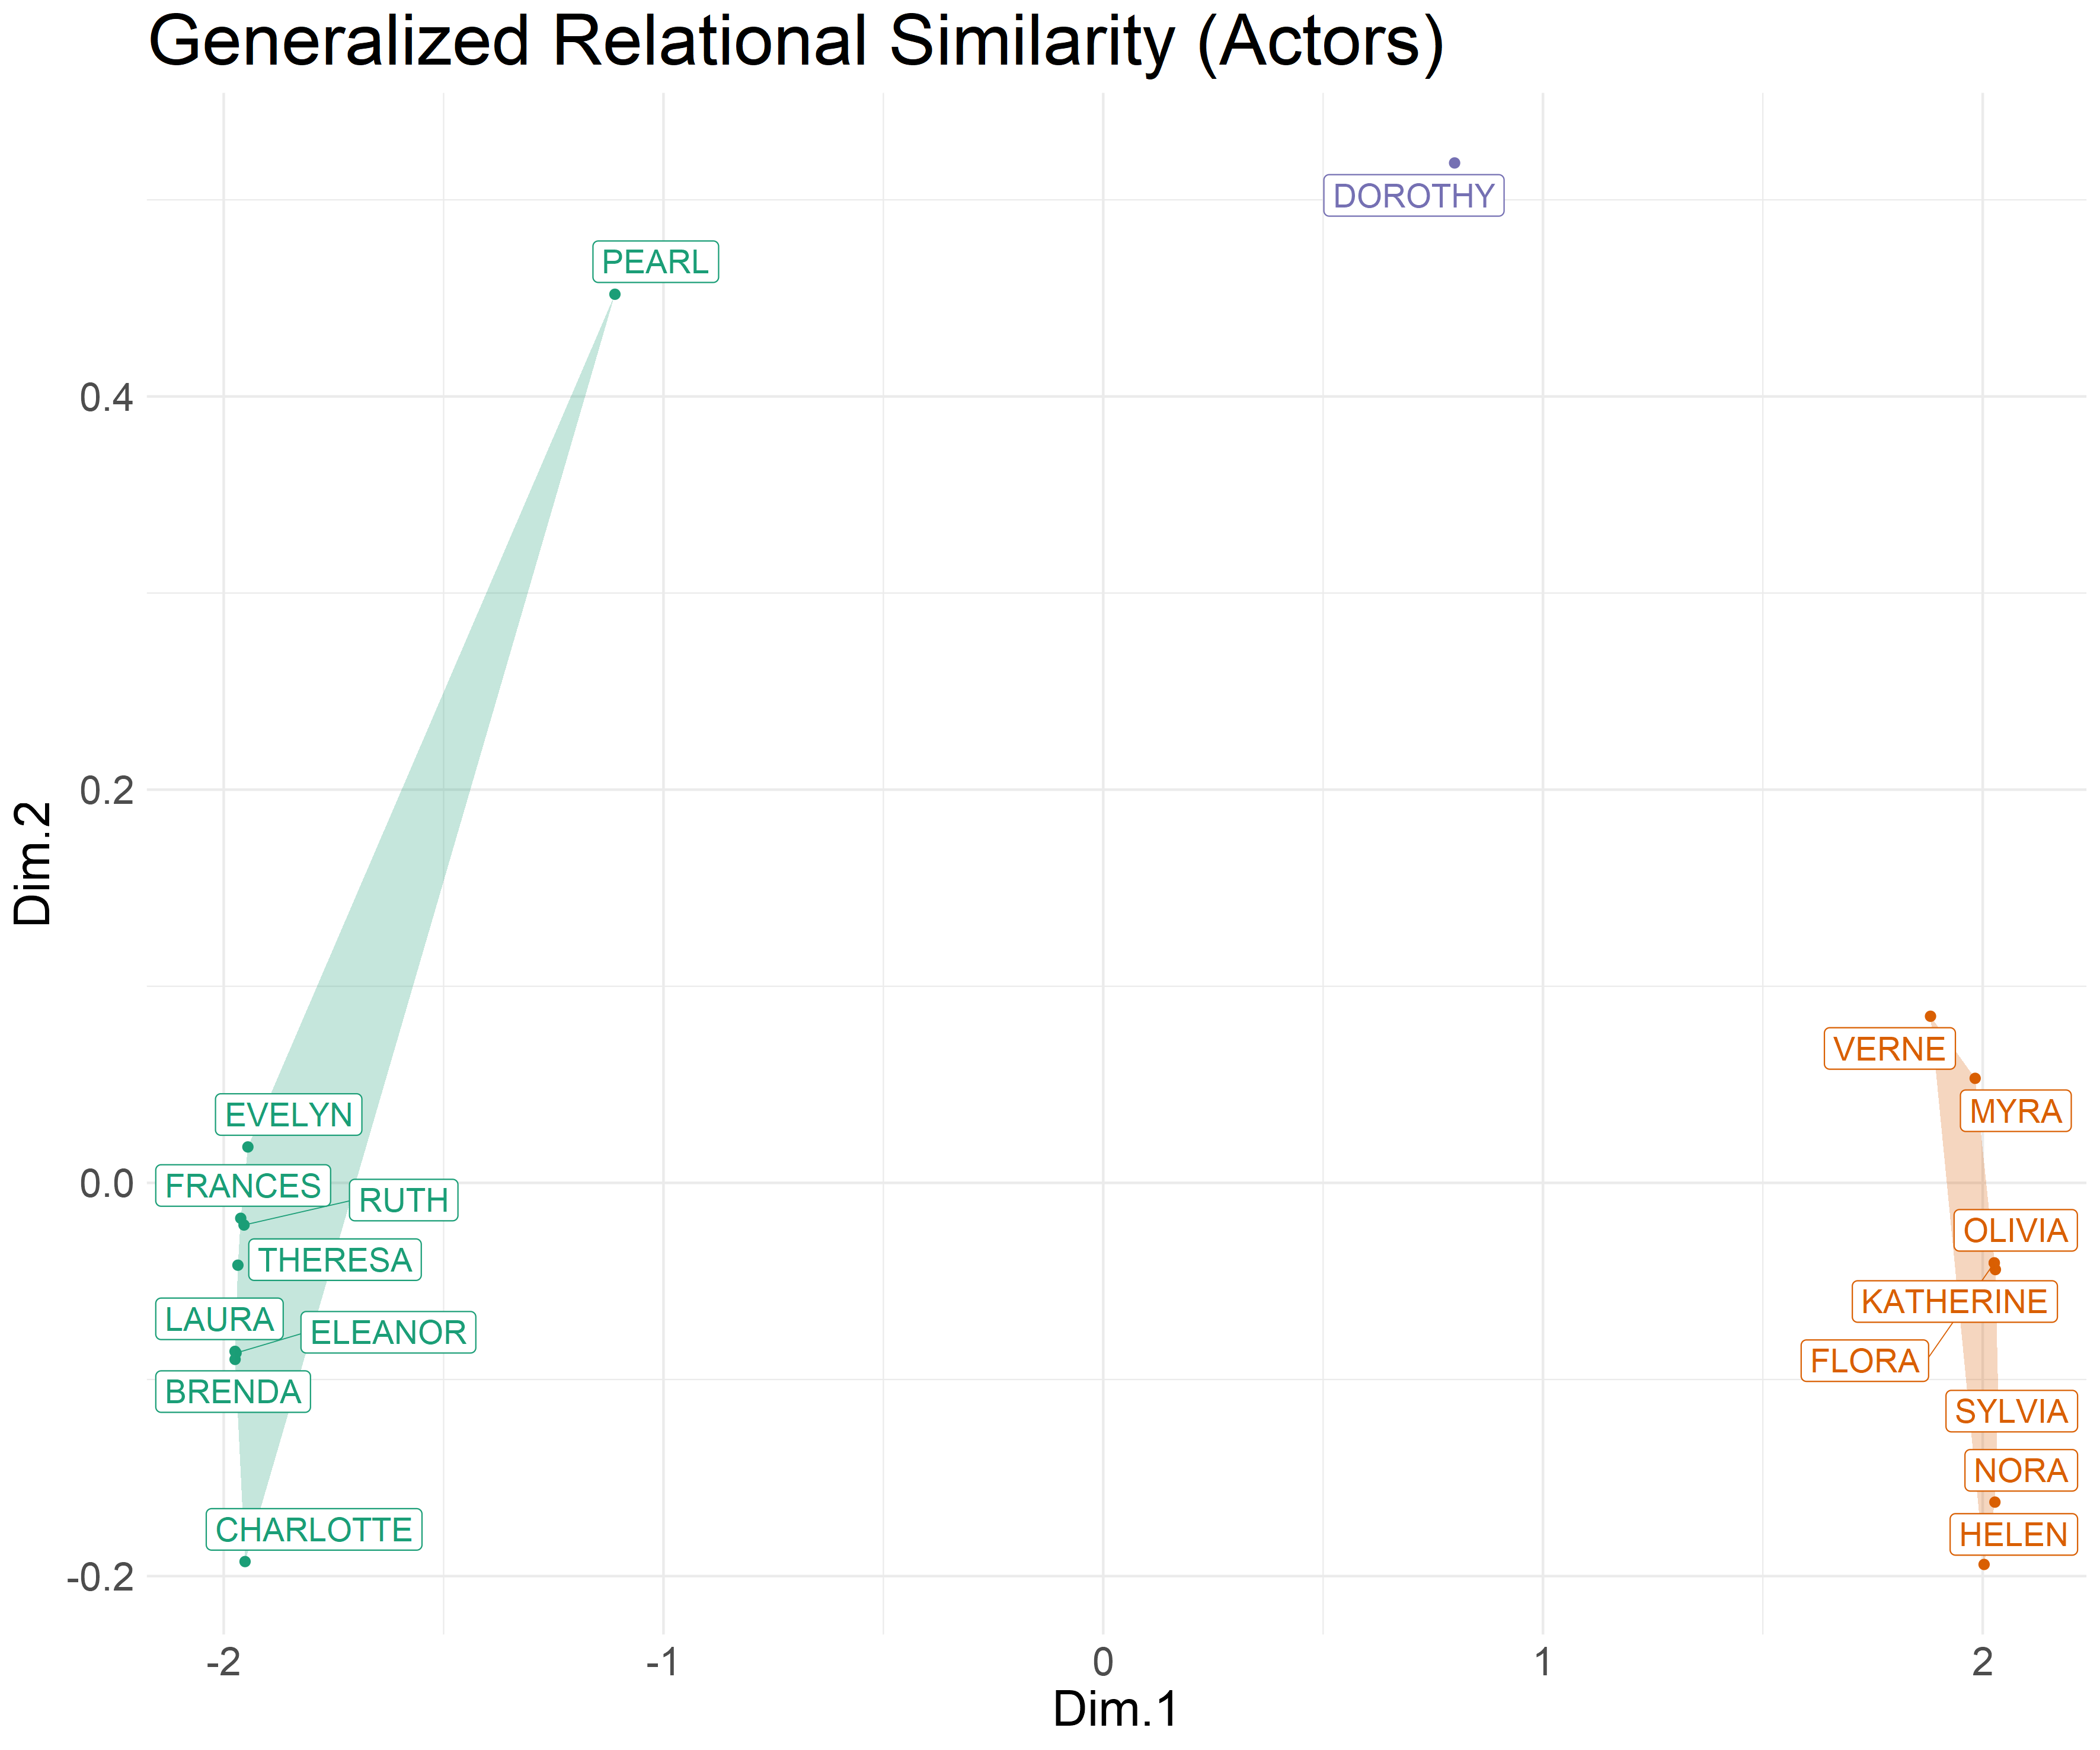
\includegraphics[width=0.7\textwidth]{Plots/grs-actors.png}
        \caption{}
        \label{fig:grm-actors}
    \end{subfigure} 
     \begin{subfigure}[b]{1.0\textwidth}
        \centering
        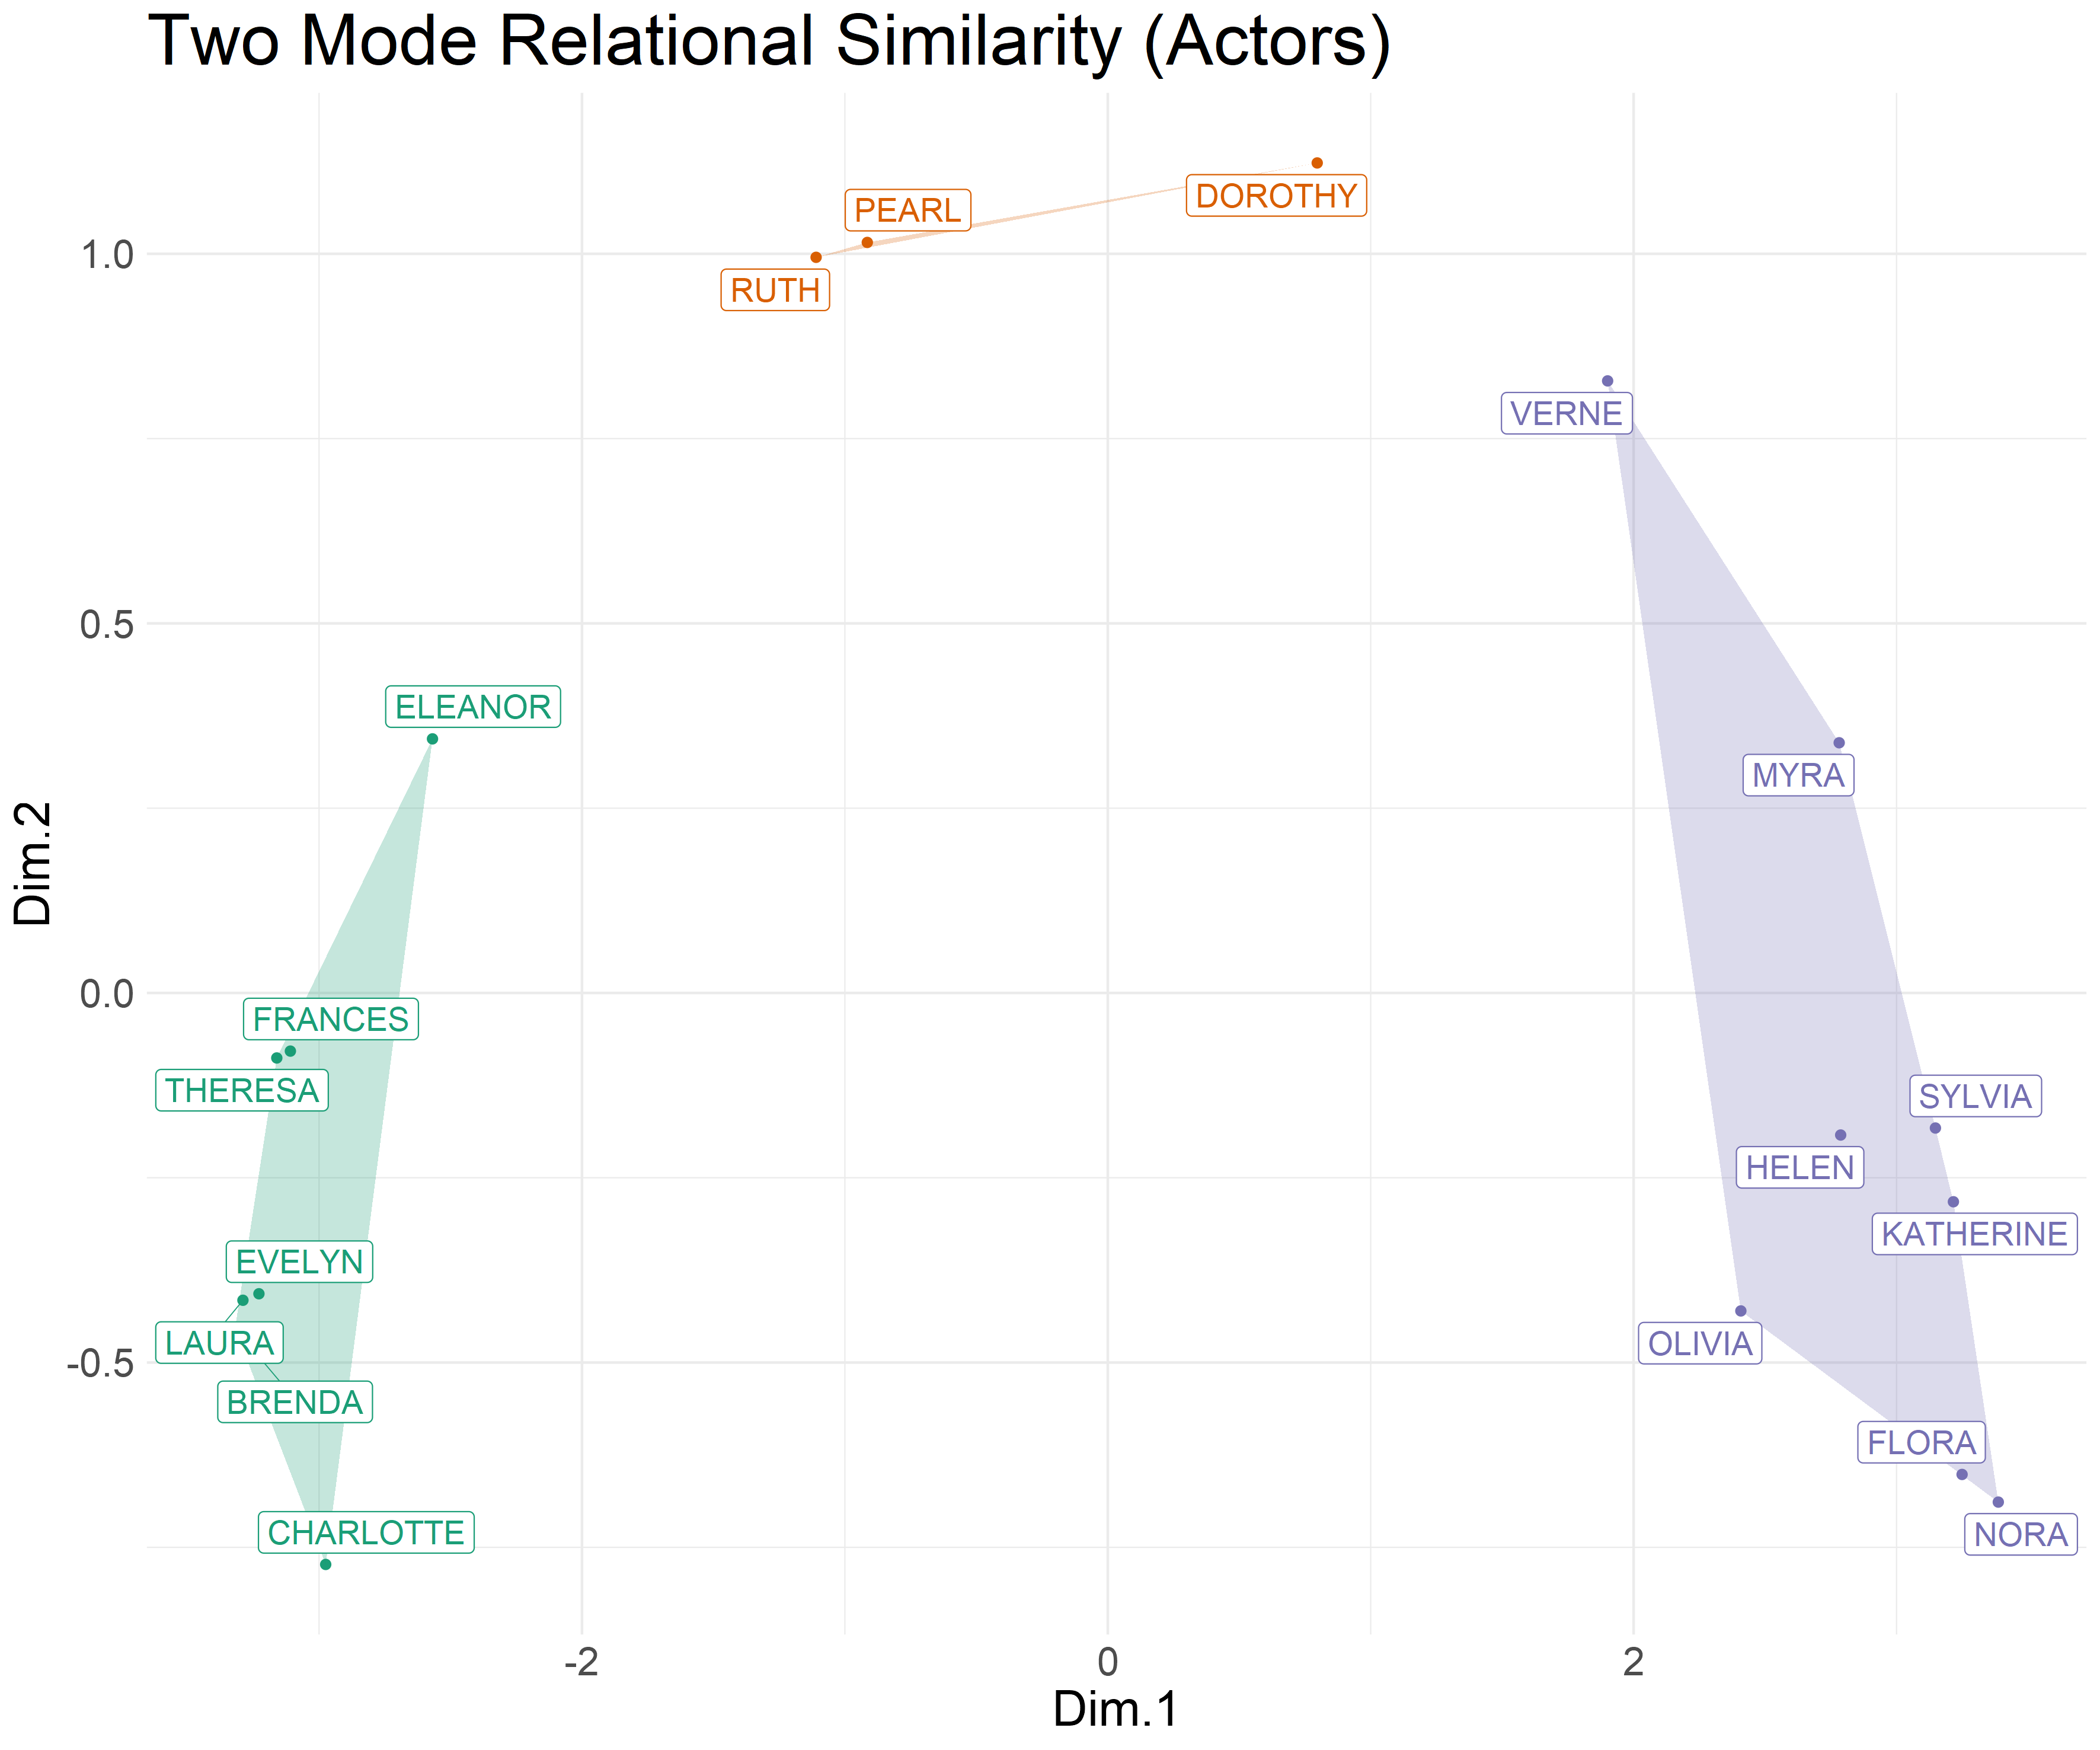
\includegraphics[width=0.7\textwidth]{Plots/tmrs-actors.png}
        \caption{}
        \label{fig:tmrs-actors}
    \end{subfigure} 
    \caption{Two-dimensional metric multidimensional scaling plots of generalized relational similarities for actors in the Southern Women data. Colors correspond to a three-group k-means clustering of the relational similarities, with cluster centroids determined by a first-step hierarchical clustering of distances according to Ward's \citeyearpar{ward63} criterion.}
    \label{fig:actors}
 \end{figure}

\section{Analysis of Southern Women Data}
In this section, I re-analyze Davis et al.'s \citeyearpar{davis1941}, Southern Women Data---also analyzed by Kovacs---showing that both Kovacs's iterated approach ($D^{grs}$) and the more direct two-mode approach ($D^{tmrs}$) yield comparable results. Like Kovacs, I take Doreian et al.'s generalized blockmodeling partitioning of actors and events as a reference point \citeyearpar[Table 4]{doreian2004}. An optimal ``unsupervised'' similarity-based partition should thus yield three clusters of actors $C_1^A =$ \{Evelyn, Laura, Theresa, Brenda, Charlotte, Frances, Eleanor, Ruth\}, $C_2^A=$ \{Verne Myra, Katherine, Sylvia, Nora, Helen, Olivia, Flora\}, and $C_3^A=$ \{Pearl, Dorothy\} and three clusters of events $C_1^E=$ \{$E_1$, $E_2$, $E_3$, $E_4$, $E_5$\}, $C_2^E=$ \{$E_6$, $E_7$, $E_8$, $E_9$\}, $C_3^E=$ \{$E_{10}$, $E_{11}$, $E_{12}$, $E_{13}$, $E_{14}$\}. 

Figures \ref{fig:actors} and \ref{fig:events} summarize the main thrust of the findings.\footnote{All plots are built using the \texttt{ggplot2} grammar of graphics \citep{wickham16}, particularly the \texttt{ggscatter} function from the package \texttt{ggpubr} \citep{kassambara}.} Like Kovacs, I present a multidimensional scaling (MDS) solution based a matrix of distances, computed as $d_{ij} = \frac{(1-s_{ij})}{2}$, where $d_{ij}$ is the distance and $s_{ij}$ is the relevant similarity between objects $i$ and $j$. 

I depart from Kovacs's original analysis in that I use a ``hybrid'' (hierarchical and k-means) clustering of the MDS distances to obtain data-driven groupings of the objects \citep{chen2005novel}, rather than just ``eyeballing'' the MDS plot. This also allows us to better detect more subtle differences in the quality of the MDS solutions---e.g., relative to \citet{doreian2004}---using the generalized relational similarities and the two-mode relational similarities. 

\subsection{Actors}
Figure \ref{fig:grm-actors} replicates Kovacs's \citeyearpar{kovacs2010} Figure 12b exactly using the author's implementation of Kovacs's algorithm written as a function for the \textit{R} statistical computing environment (see Supplementary materials). After twelve iterations, the algorithm converged (using $\epsilon = 0.001$). 

As Kovacs noted, the distribution of points in the two-dimensional MDS space obtained using the generalized relational similarities corresponds to the generalized blockmodeling solution reported by \citet{doreian2004}, with two large sets of similar actors separated from one another and the more peripheral Dorothy and Pearl. Note however, that using the generalized relational similarity approach, the k-means clustering misclassifies Pearl as belonging to the first large cluster and puts Dorothy in her own singleton cluster. 

As Figure~\ref{fig:tmrs-actors} shows, the two-mode relational similarity approach yields comparable results to Kovacs's generalized relational similarities, also revealing Doreian et al.'s actor blocks. Notably, the k-means three-cluster solution for the two-mode relational similarities correctly assigns Pearl and Dorothy to their own cluster, thus coming closer to Doreian et al.'s generalized blockmodeling results than Kovacs's generalized relationality similarity. 

  \begin{figure}[ht!]
     \begin{subfigure}[b]{1.0\textwidth}
        \centering
        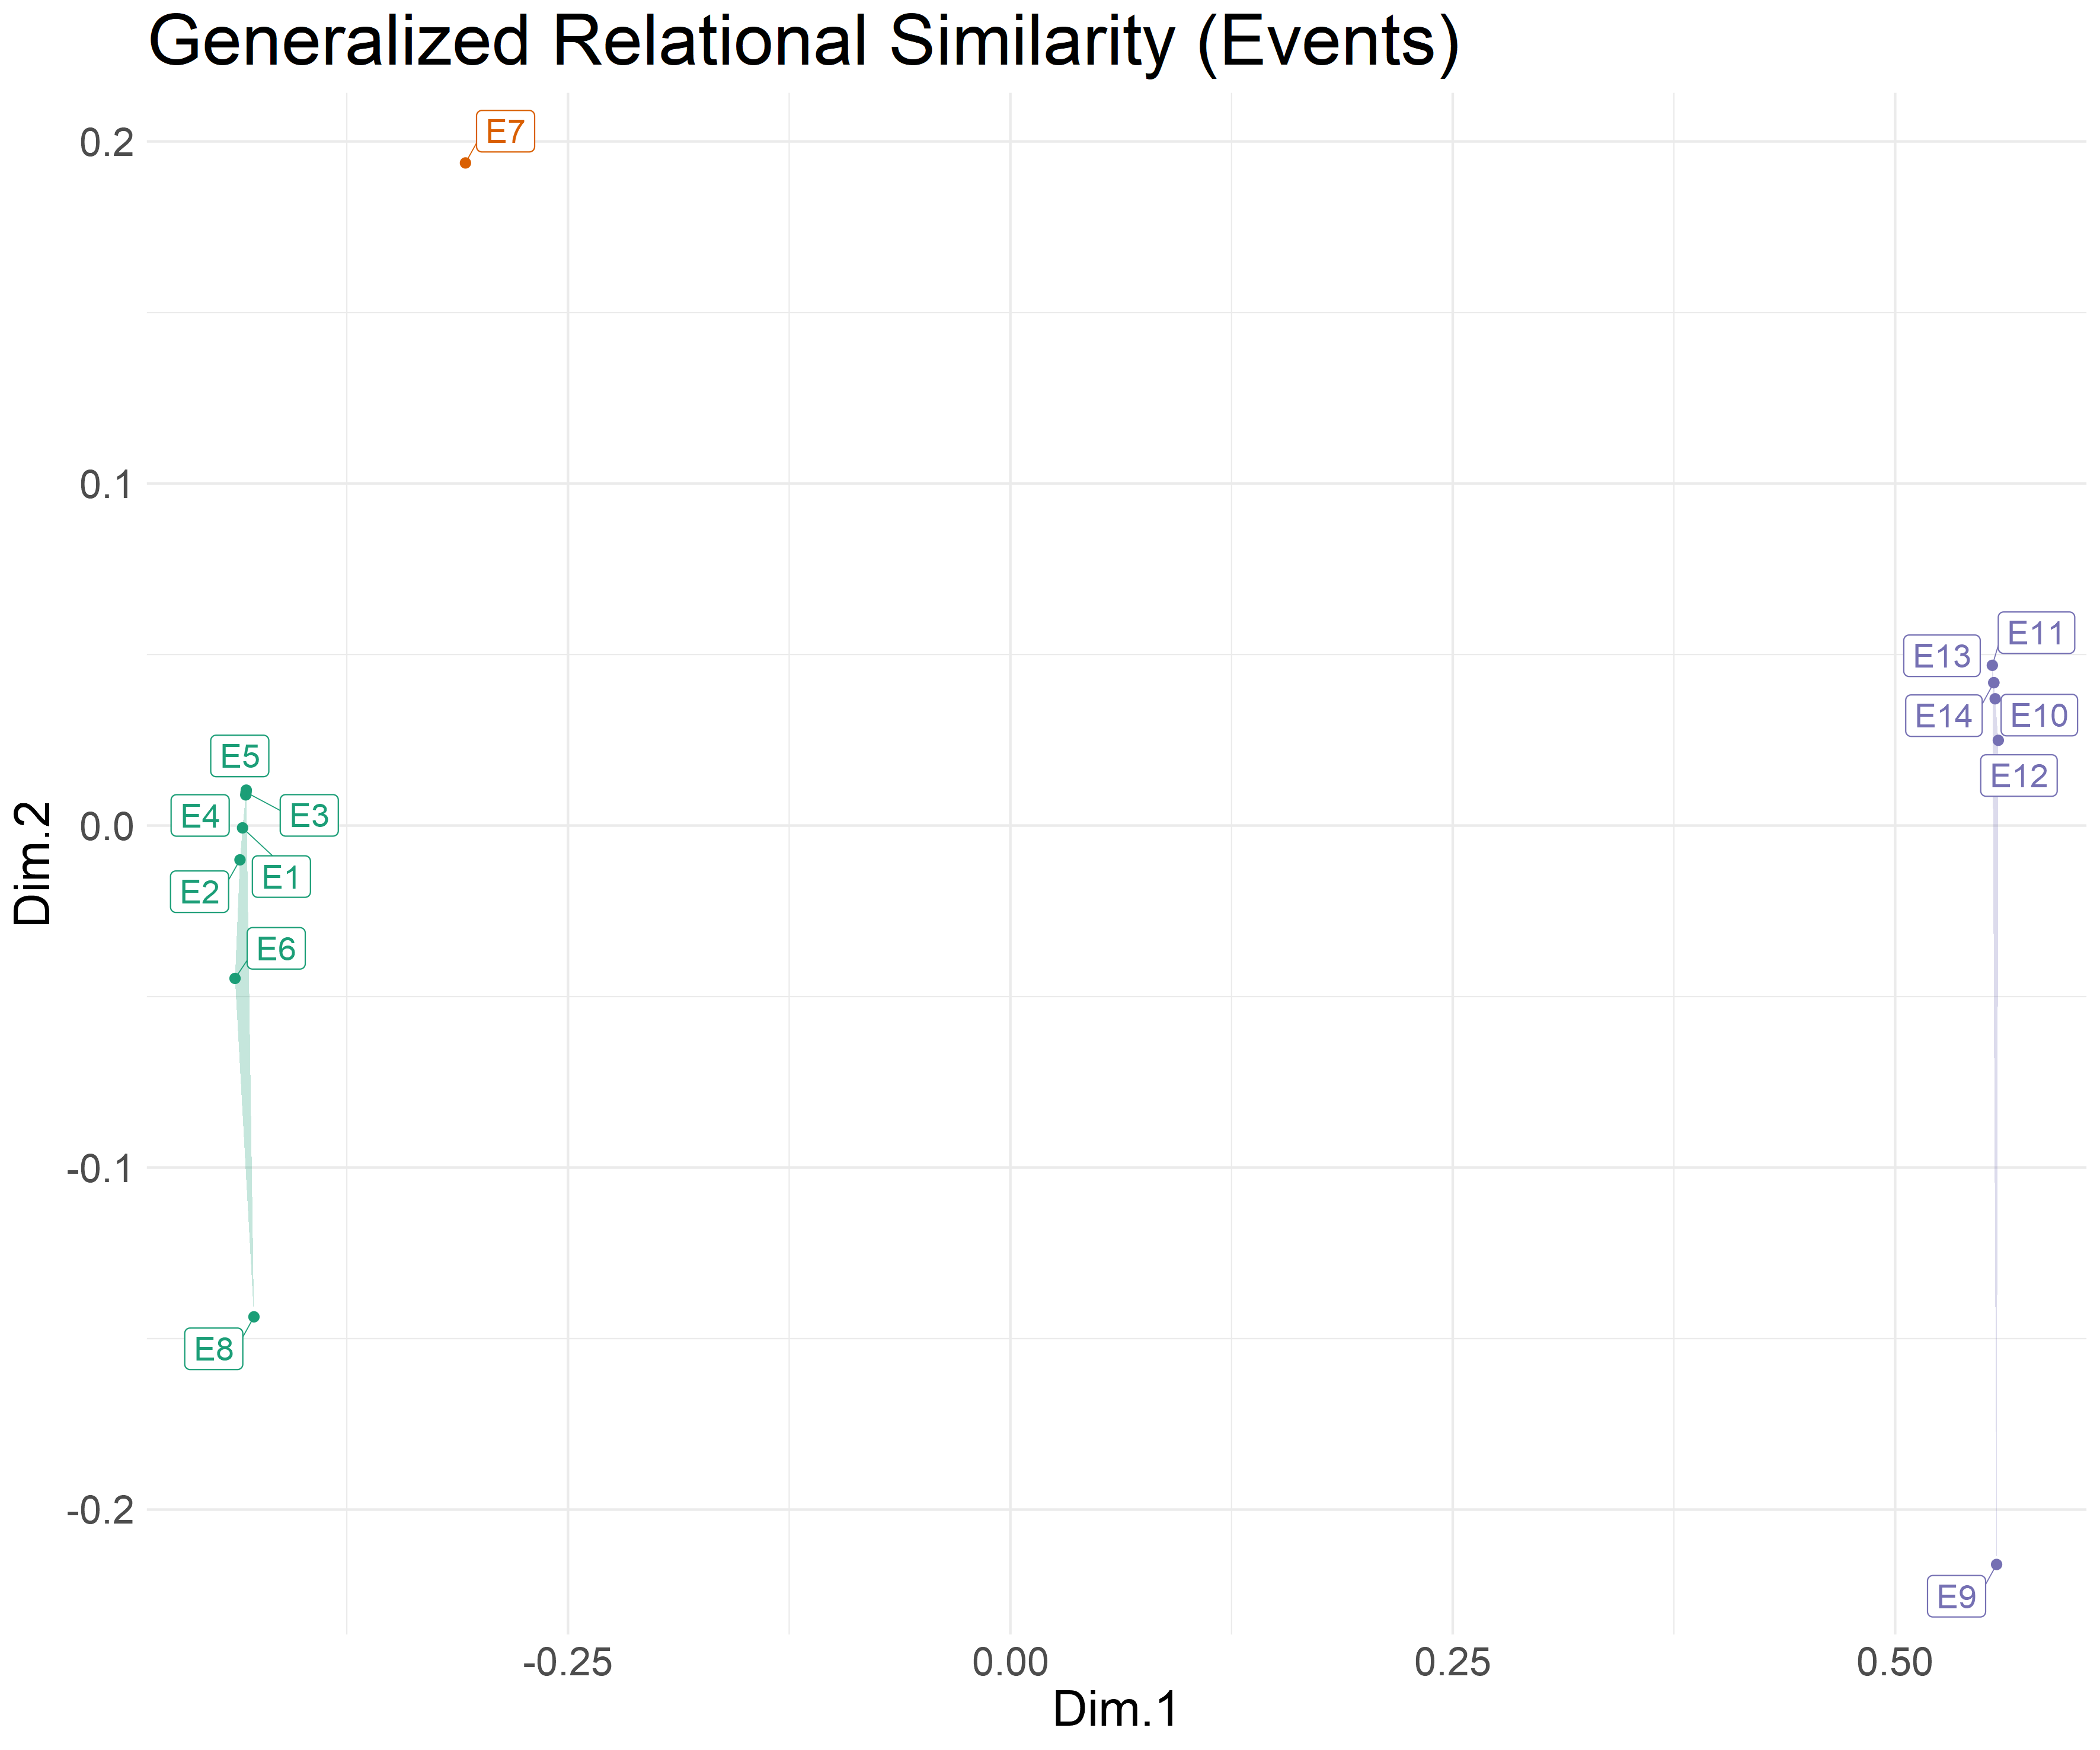
\includegraphics[width=0.7\textwidth]{Plots/grs-events.png}
        \caption{}
        \label{fig:grm-events}
    \end{subfigure} 
     \begin{subfigure}[b]{1.0\textwidth}
        \centering
        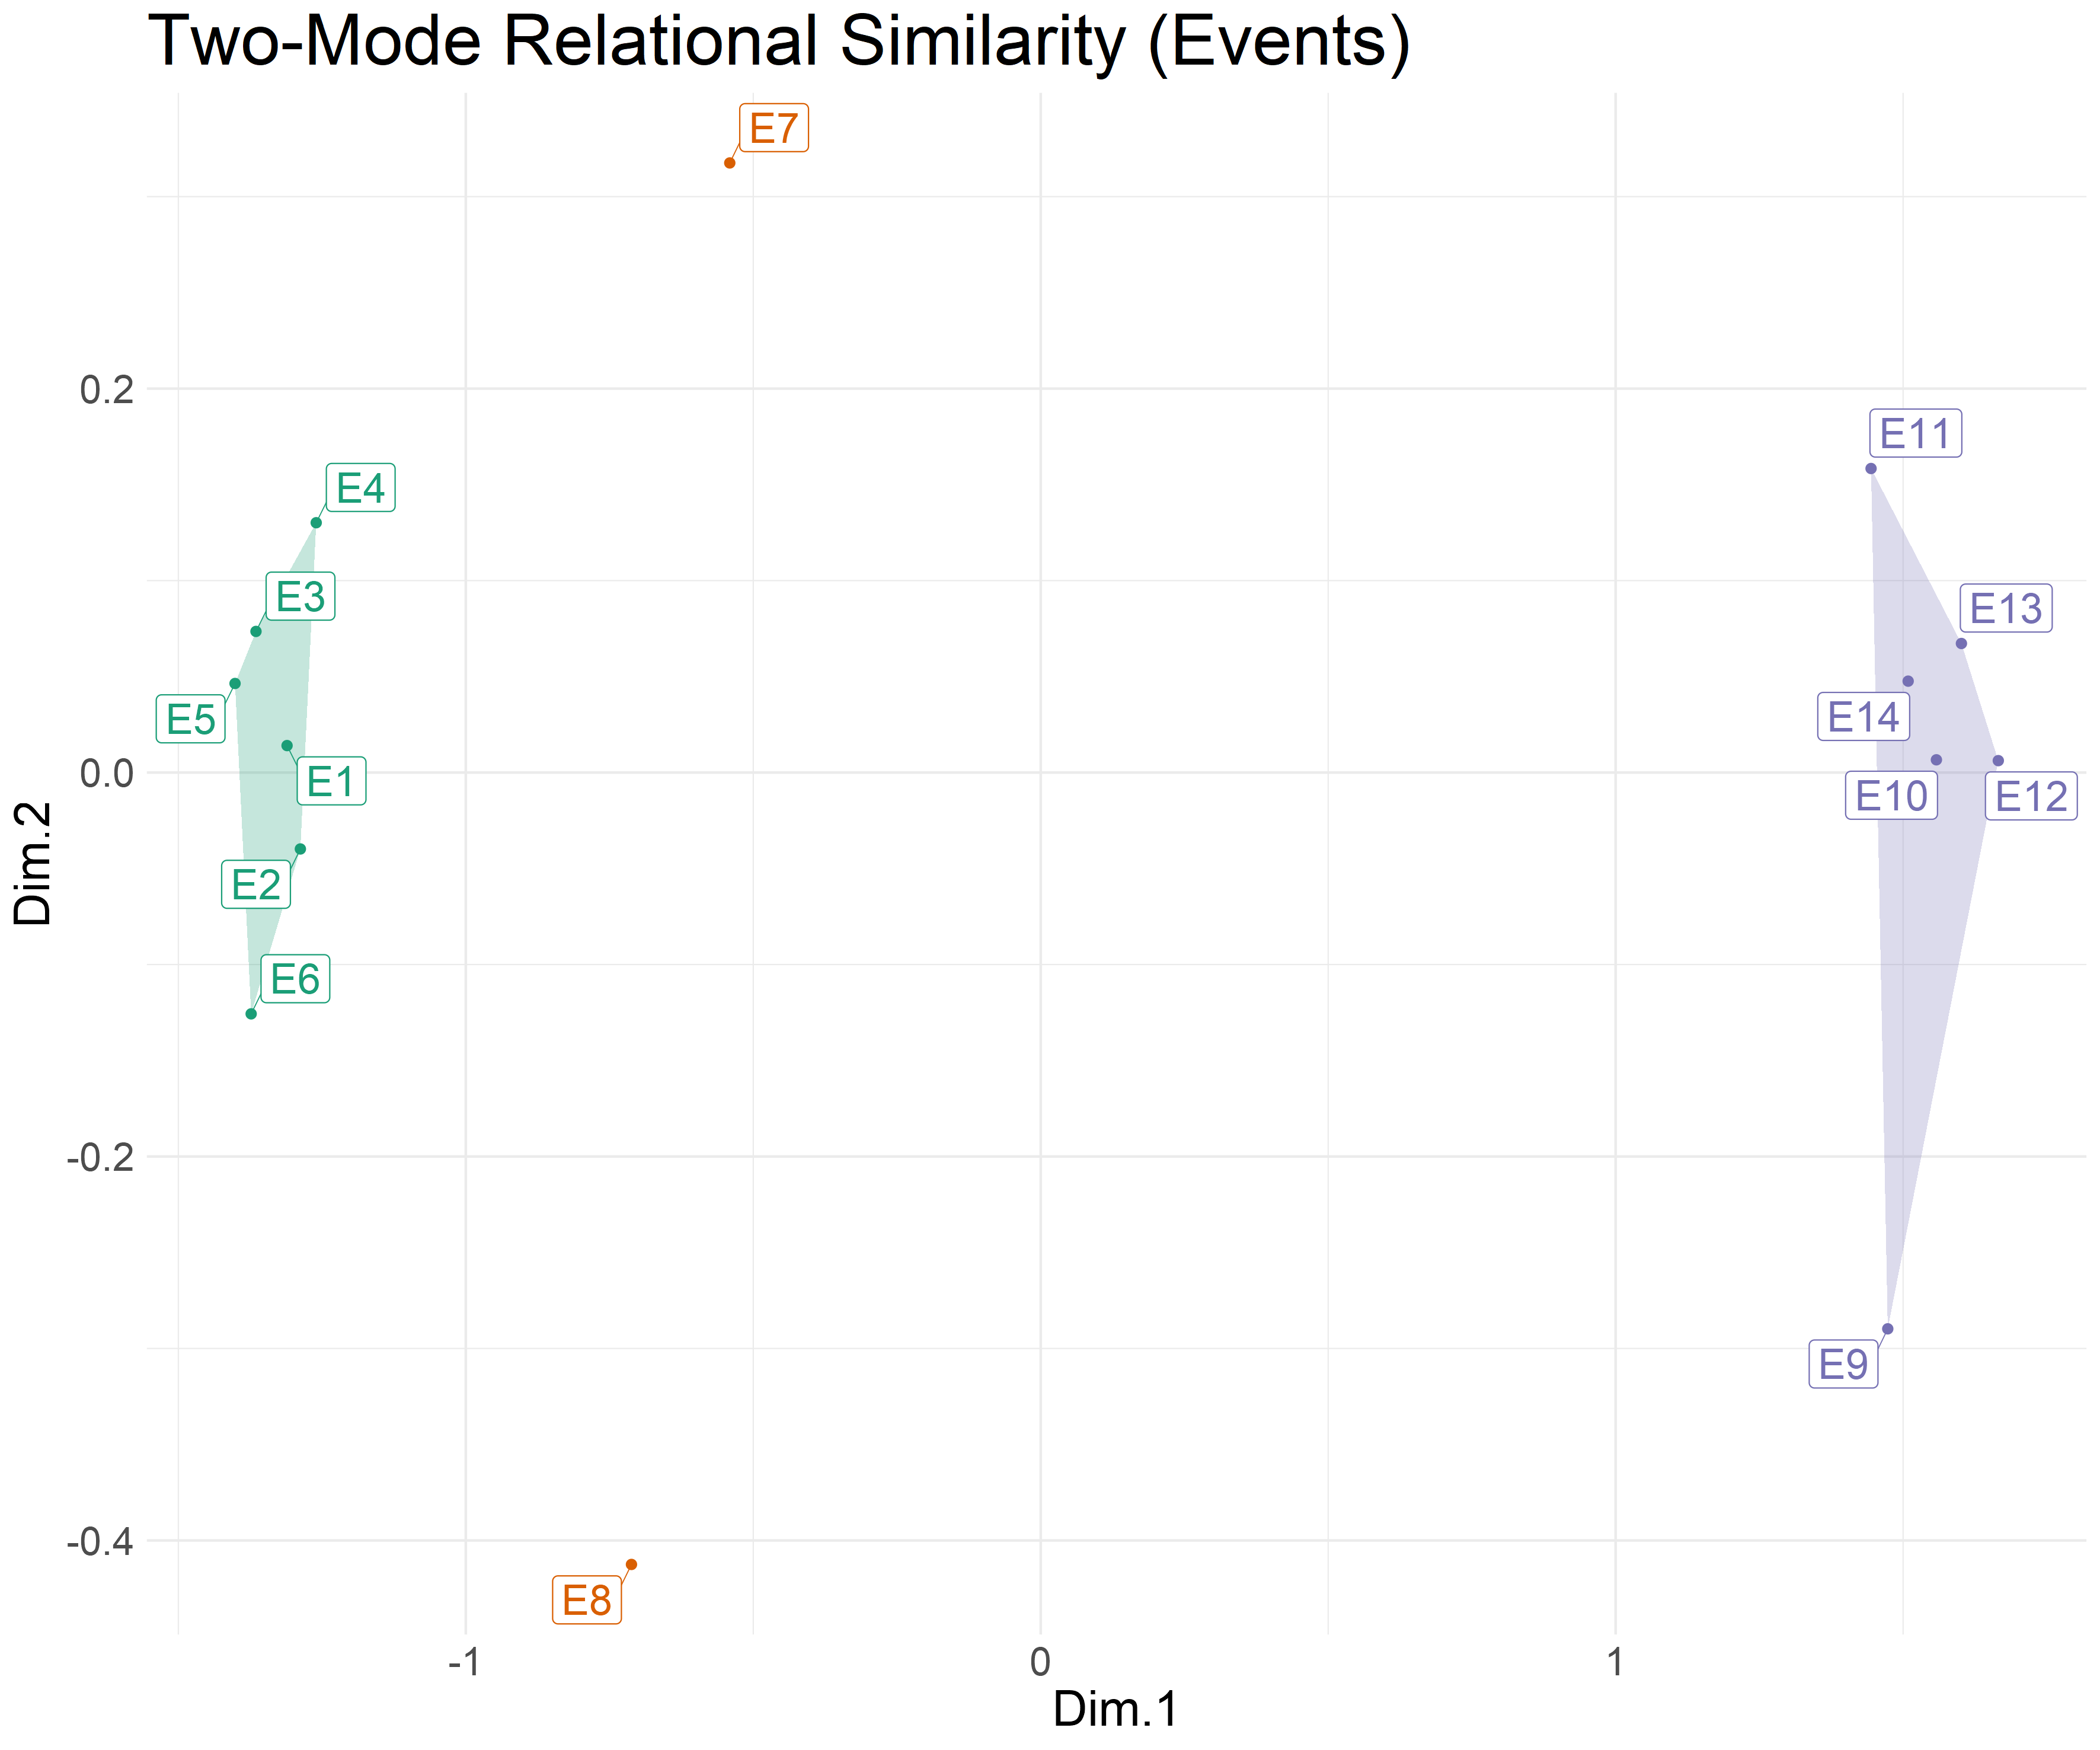
\includegraphics[width=0.7\textwidth]{Plots/tmrs-events.png}
        \caption{}
        \label{fig:tmrs-events}
    \end{subfigure} 
    \caption{Two-dimensional metric multidimensional scaling plots of generalized relational similarities for events in the Southern Women data. Colors correspond to a five-group k-means clustering of the relational similarities, with cluster centroids determined by a first-step hierarchical clustering according to Ward's \citeyearpar{ward63} criterion.}
    \label{fig:events}
 \end{figure}

\subsection{Events}
Figure \ref{fig:events} reports the corresponding analysis for relational similarities of the object (events). In the original paper, Kovacs \citeyearpar[206]{kovacs2010}, described these results verbally---no plot was provided---as follows:

\begin{quote}
The generalized similarity model provides a grouping for the events as well (not shown here). This grouping differs slightly from Doreian et al.'s \citeyearpar{doreian2004} grouping: although the (1, 2, 3, 4, 5) and (10, 11, 12, 13, 14) clusters emerge in the generalized similarity solution as well, the picture differs for events 6, 7, 8, and 9. Event 6 here is clustered together with (1, 2, 3, 4, 5), while events 7, 8 and 9 do not fall into any group but stand separately  (206). 
\end{quote}

Figure~\ref{fig:grm-events} replicates Kocacs's verbal description of the results using generalized relational similarities. A three-group k-means clustering of the distances in the multidimensional scaling space separates the closely-spaced events 1-6 and 10-14. Event 7 is assigned to its own singleton cluster, and events 8 and 9 are assigned to the events 1-6 and events 10-14 clusters respectively. 

As Figure~\ref{fig:tmrs-events} shows, the two-mode relational similarity approach yields results that are somewhat different from those obtained using the generalized relational similarities, but that are in some ways closer to the target clusters from Doreian et al.'s blockmodel solution \citeyearpar{doreian2004}. As with the Kovacs approach, events 1-6 and events 10-14 end up closely spaced and assigned to their own cluster. Events 7 and 8 fall into their own cluster as would be expected given the Doreian et al. partition. Event 9, however, is grouped with the event 10-14 cluster. In all, the two-mode relational similarity approach seems more effective at avoiding singleton clusters than than the generalized similarity measure. 

\section{Conclusion}
Kovacs \citeyearpar{kovacs2010} made a case that a desirable metric for relational similarity should respect at least two basic desiderata, which I have referred to as the principles of equivalence and duality, proposing an approach based on iterated correlations that met these criteria. In this short note, I have shown that we can get there using a more straightforward, non-iterative approach, more directly grounded in the principle of duality via the dual projection approach to analyzing two-mode data \citep{everett2013}. 

Like Kovacs, this approach tunes the correlation distances between entities in one mode based on their connection to similar entities in the other mode, as revealed by the one-mode projections. A replication of Kovacs's analysis of Davis et al.'s \citeyearpar{davis1941} Southern Women Data and a re-analysis based on the proposed alternative metric shows that the two-mode relational similarity approach yields substantively identical results to those obtained using the generalized similarity strategy. 

%% Loading bibliography style file
%\bibliographystyle{model1-num-names}
\bibliographystyle{cas-model2-names}
% Loading bibliography database
\bibliography{cas-refs}
\end{document}


The Elsevier cas-dc class is based on the
standard article class and supports almost all of the functionality of
that class. In addition, it features commands and options to format the
\begin{itemize} \item document style \item baselineskip \item front
matter \item keywords and MSC codes \item theorems, definitions and
proofs \item lables of enumerations \item citation style and labeling.
\end{itemize}

This class depends on the following packages
for its proper functioning:

\begin{enumerate}
\itemsep=0pt
\item {natbib.sty} for citation processing;
\item {geometry.sty} for margin settings;
\item {fleqn.clo} for left aligned equations;
\item {graphicx.sty} for graphics inclusion;
\item {hyperref.sty} optional packages if hyperlinking is
  required in the document;
\end{enumerate}  

All the above packages are part of any
standard \LaTeX{} installation.
Therefore, the users need not be
bothered about downloading any extra packages.

\section{Installation}

The package is available at author resources page at Elsevier
(\url{http://www.elsevier.com/locate/latex}).
The class may be moved or copied to a place, usually,\linebreak
\verb+$TEXMF/tex/latex/elsevier/+, %$%%%%%%%%%%%%%%%%%%%%%%%%%%%%
or a folder which will be read                   
by \LaTeX{} during document compilation.  The \TeX{} file
database needs updation after moving/copying class file.  Usually,
we use commands like \verb+mktexlsr+ or \verb+texhash+ depending
upon the distribution and operating system.

\section{Front matter}

The author names and affiliations could be formatted in two ways:
\begin{enumerate}[(1)]
\item Group the authors per affiliation.
\item Use footnotes to indicate the affiliations.
\end{enumerate}
See the front matter of this document for examples. 
You are recommended to conform your choice to the journal you 
are submitting to.

\section{Bibliography styles}

There are various bibliography styles available. You can select the
style of your choice in the preamble of this document. These styles are
Elsevier styles based on standard styles like Harvard and Vancouver.
Please use Bib\TeX\ to generate your bibliography and include DOIs
whenever available.

Here are two sample references: 
\cite{Fortunato2010}
\cite{Fortunato2010,NewmanGirvan2004}
\cite{Fortunato2010,Vehlowetal2013}

\section{Floats}
{Figures} may be included using the command,\linebreak 
\verb+\includegraphics+ in
combination with or without its several options to further control
graphic. \verb+\includegraphics+ is provided by {graphic[s,x].sty}
which is part of any standard \LaTeX{} distribution.
{graphicx.sty} is loaded by default. \LaTeX{} accepts figures in
the postscript format while pdf\LaTeX{} accepts {*.pdf},
{*.mps} (metapost), {*.jpg} and {*.png} formats. 
pdf\LaTeX{} does not accept graphic files in the postscript format. 

\begin{figure}
	\centering
		
\includegraphics[scale=.75]{figs/Fig1.pdf}
	\caption{The evanescent light - $1S$ quadrupole coupling
	($g_{1,l}$) scaled to the bulk exciton-photon coupling
	($g_{1,2}$). The size parameter $kr_{0}$ is denoted as $x$ and
	the \PMS is placed directly on the cuprous oxide sample ($\delta
	r=0$, See also Table \protect\ref{tbl1}).}
	\label{FIG:1}
\end{figure}


The \verb+table+ environment is handy for marking up tabular
material. If users want to use {multirow.sty},
{array.sty}, etc., to fine control/enhance the tables, they
are welcome to load any package of their choice and
{cas-dc.cls} will work in combination with all loaded
packages.

\begin{table}[width=.9\linewidth,cols=4,pos=h]
\caption{This is a test caption. This is a test caption. This is a test
caption. This is a test caption.}\label{tbl1}
\begin{tabular*}{\tblwidth}{@{} LLLL@{} }
\toprule
Col 1 & Col 2 & Col 3 & Col4\\
\midrule
12345 & 12345 & 123 & 12345 \\
12345 & 12345 & 123 & 12345 \\
12345 & 12345 & 123 & 12345 \\
12345 & 12345 & 123 & 12345 \\
12345 & 12345 & 123 & 12345 \\
\bottomrule
\end{tabular*}
\end{table}

\section[Theorem and ...]{Theorem and theorem like environments}

{cas-dc.cls} provides a few shortcuts to format theorems and
theorem-like environments with ease. In all commands the options that
are used with the \verb+\newtheorem+ command will work exactly in the same
manner. {cas-dc.cls} provides three commands to format theorem or
theorem-like environments: 

\begin{verbatim}
 \newtheorem{theorem}{Theorem}
 \newtheorem{lemma}[theorem]{Lemma}
 \newdefinition{rmk}{Remark}
 \newproof{pf}{Proof}
 \newproof{pot}{Proof of Theorem \ref{thm2}}
\end{verbatim}


The \verb+\newtheorem+ command formats a
theorem in \LaTeX's default style with italicized font, bold font
for theorem heading and theorem number at the right hand side of the
theorem heading.  It also optionally accepts an argument which
will be printed as an extra heading in parentheses. 

\begin{verbatim}
  \begin{theorem} 
   For system (8), consensus can be achieved with 
   $\|T_{\omega z}$ ...
     \begin{eqnarray}\label{10}
     ....
     \end{eqnarray}
  \end{theorem}
\end{verbatim}  


\newtheorem{theorem}{Theorem}

\begin{theorem}
For system (8), consensus can be achieved with 
$\|T_{\omega z}$ ...
\begin{eqnarray}\label{10}
....
\end{eqnarray}
\end{theorem}

The \verb+\newdefinition+ command is the same in
all respects as its \verb+\newtheorem+ counterpart except that
the font shape is roman instead of italic.  Both
\verb+\newdefinition+ and \verb+\newtheorem+ commands
automatically define counters for the environments defined.

The \verb+\newproof+ command defines proof environments with
upright font shape.  No counters are defined. 


\section[Enumerated ...]{Enumerated and Itemized Lists}
{cas-dc.cls} provides an extended list processing macros
which makes the usage a bit more user friendly than the default
\LaTeX{} list macros.   With an optional argument to the
\verb+\begin{enumerate}+ command, you can change the list counter
type and its attributes.

\begin{verbatim}
 \begin{enumerate}[1.]
 \item The enumerate environment starts with an optional
   argument `1.', so that the item counter will be suffixed
   by a period.
 \item You can use `a)' for alphabetical counter and '(i)' 
  for roman counter.
  \begin{enumerate}[a)]
    \item Another level of list with alphabetical counter.
    \item One more item before we start another.
    \item One more item before we start another.
    \item One more item before we start another.
    \item One more item before we start another.
\end{verbatim}

Further, the enhanced list environment allows one to prefix a
string like `step' to all the item numbers.  

\begin{verbatim}
 \begin{enumerate}[Step 1.]
  \item This is the first step of the example list.
  \item Obviously this is the second step.
  \item The final step to wind up this example.
 \end{enumerate}
\end{verbatim}

\section{Cross-references}
In electronic publications, articles may be internally
hyperlinked. Hyperlinks are generated from proper
cross-references in the article.  For example, the words
\textcolor{black!80}{Fig.~1} will never be more than simple text,
whereas the proper cross-reference \verb+\ref{tiger}+ may be
turned into a hyperlink to the figure itself:
\textcolor{blue}{Fig.~1}.  In the same way,
the words \textcolor{blue}{Ref.~[1]} will fail to turn into a
hyperlink; the proper cross-reference is \verb+\cite{Knuth96}+.
Cross-referencing is possible in \LaTeX{} for sections,
subsections, formulae, figures, tables, and literature
references.

\section{Bibliography}

Two bibliographic style files (\verb+*.bst+) are provided ---
{model1-num-names.bst} and {model2-names.bst} --- the first one can be
used for the numbered scheme. This can also be used for the numbered
with new options of {natbib.sty}. The second one is for the author year
scheme. When  you use model2-names.bst, the citation commands will be
like \verb+\citep+,  \verb+\citet+, \verb+\citealt+ etc. However when
you use model1-num-names.bst, you may use only \verb+\cite+ command.

\verb+thebibliography+ environment.  Each reference is a\linebreak
\verb+\bibitem+ and each \verb+\bibitem+ is identified by a label,
by which it can be cited in the text:

\noindent In connection with cross-referencing and
possible future hyperlinking it is not a good idea to collect
more that one literature item in one \verb+\bibitem+.  The
so-called Harvard or author-year style of referencing is enabled
by the \LaTeX{} package {natbib}. With this package the
literature can be cited as follows:

\begin{enumerate}[\textbullet]
\item Parenthetical: \verb+\citep{WB96}+ produces (Wettig \& Brown, 1996).
\item Textual: \verb+\citet{ESG96}+ produces Elson et al. (1996).
\item An affix and part of a reference:\break
\verb+\citep[e.g.][Ch. 2]{Gea97}+ produces (e.g. Governato et
al., 1997, Ch. 2).
\end{enumerate}

In the numbered scheme of citation, \verb+\cite{<label>}+ is used,
since \verb+\citep+ or \verb+\citet+ has no relevance in the numbered
scheme.  {natbib} package is loaded by {cas-dc} with
\verb+numbers+ as default option.  You can change this to author-year
or harvard scheme by adding option \verb+authoryear+ in the class
loading command.  If you want to use more options of the {natbib}
package, you can do so with the \verb+\biboptions+ command.  For
details of various options of the {natbib} package, please take a
look at the {natbib} documentation, which is part of any standard
\LaTeX{} installation.

\appendix
\section{My Appendix}
Appendix sections are coded under \verb+\appendix+.

\verb+\printcredits+ command is used after appendix sections to list 
author credit taxonomy contribution roles tagged using \verb+\credit+ 
in frontmatter.

\printcredits




%\vskip3pt

\bio{}
Author biography without author photo.
Author biography. Author biography. Author biography.
Author biography. Author biography. Author biography.
Author biography. Author biography. Author biography.
Author biography. Author biography. Author biography.
Author biography. Author biography. Author biography.
Author biography. Author biography. Author biography.
Author biography. Author biography. Author biography.
Author biography. Author biography. Author biography.
Author biography. Author biography. Author biography.
\endbio

\bio{figs/pic1}
Author biography with author photo.
Author biography. Author biography. Author biography.
Author biography. Author biography. Author biography.
Author biography. Author biography. Author biography.
Author biography. Author biography. Author biography.
Author biography. Author biography. Author biography.
Author biography. Author biography. Author biography.
Author biography. Author biography. Author biography.
Author biography. Author biography. Author biography.
Author biography. Author biography. Author biography.
\endbio

\bio{figs/pic1}
Author biography with author photo.
Author biography. Author biography. Author biography.
Author biography. Author biography. Author biography.
Author biography. Author biography. Author biography.
Author biography. Author biography. Author biography.
\endbio

